Le contromisure possibili possono essere classificate come contromisure “a monte” e “a valle”.\\
“A monte” abbiamo:
\begin{itemize}
\item[-] la possibilità di disattivare gli script .ida e .idq nel caso in cui non fossero necessari;
\item[-] cambiare indirizzo IP per evitare l’attacco DDoS. Nello specifico è stata la soluzione adottata dalla Casa Bianca al momento dell’attacco;
\item[-] il download della patch che va ad inserire il controllo sull’input mancante, in modo da eliminare completamente la vulnerabilità presente.
\end{itemize}
“A valle” ci sono invece dei prodotti software utili per scansionare il dispositivo ed eventualmente eliminare il worm trovato. Questi sono “FixCodeRed” rilasciato dalla Symantec e “CodeRedScanner” rilasciato proprio dalla Eye Digital Security.\\
Queste contromisure sono state effettivamente adottate nel periodo dell’attacco e hanno contribuito, almeno in parte, alla riduzione della diffusione e delle conseguenze dell’attacco. Non sono però le uniche contromisure valide, anzi ce ne sono altre che avrebbero avuto un ottimo impatto nella difesa da Code Red, alcune delle quali ne avrebbero addirittura impedito una diffusione così elevata.\\
Le contromisure che abbiamo individuato sono state:
\begin{enumerate}
\item Contenimento automatizzato dei worm
\item SSL - Security Socket Layer
\item ACL - Access Control List
\item Reverse Proxy
\item IDS - Intrusion Detection System
\item WAF - Web Application Firewall
\end{enumerate}
%%%%%%%%%%%%%%%%%%%%%%%%%%%%%%%%%%%%%%%%%%%%%%%%%%%%%%%%%%%%%%%%%%%%%%%%%%%%%
\subsection{Contenimento automatizzato dei worm}
Il contenimento automatizzato è una tecnica ideata dai ricercatori Sellke, Shroff e Bagchi~\cite{selke} che consiste nel blocco o nel rallentamento della comunicazione tra host infetti e host non infetti, impedendo ad un generico worm a scansione randomica di diffondersi sin dalle prime fasi del contagio.\\
L’idea principale è quella di limitare il numero totale di distinti indirizzi IP contattati da un singolo host nell’arco di un lungo periodo di tempo (settimane o anche giorni), detto ciclo di contenimento, in modo tale da ottenere una probabilità di estinzione $\pi$ prossima a 1.\\
La seguente proposizione fornisce la condizione necessaria e sufficiente affinché l’estinzione si verifichi con certezza:\\
%%%%%%%%
\newtheorem{prop}{Proposizione}
\begin{prop}
Sia p la densità di probabilità degli host suscettibili e M il numero massimo di scansioni per host, allora:
\begin{displaymath}
    \pi = 1  \Leftrightarrow  M \le 1/p 
\end{displaymath}
\end{prop}
%%%%%%%%%
L’implicazione pratica di questa proposizione è che limitando il numero totale di scansioni per host a non più di $1/p$, la diffusione del worm sarà eventualmente contenuta entro un certo numero di generazioni.\\
La densità $p$ è la probabilità di trovare un host vulnerabile ad ogni scansione ed è pari a $V/232$ dove $V$ corrisponde al numero di host vulnerabili e $2^{32}$ è la dimensione dello spazio degli indirizzi IPv4.\\
Se si assume per semplicità che il numero di host vulnerabili a Code Red era almeno di $360000$ unità, si ottiene un valore di $p$ pari a $8.5 x 10^{-5}$, e di conseguenza il numero massimo di scansioni $M$ è pari a $11930$.
La figura~\ref{auto} mostra i risultati dello studio di Selke et al. in cui si evidenzia come con un valore di $M = 10000$, il numero totale di host infetti risulti essere inferiore a $360$ unità con una probabilità del 99\%, tale numero corrisponde a circa lo 0.1\% del totale degli host vulnerabili all’epoca.\\
\begin{figure}[!h]
\centering
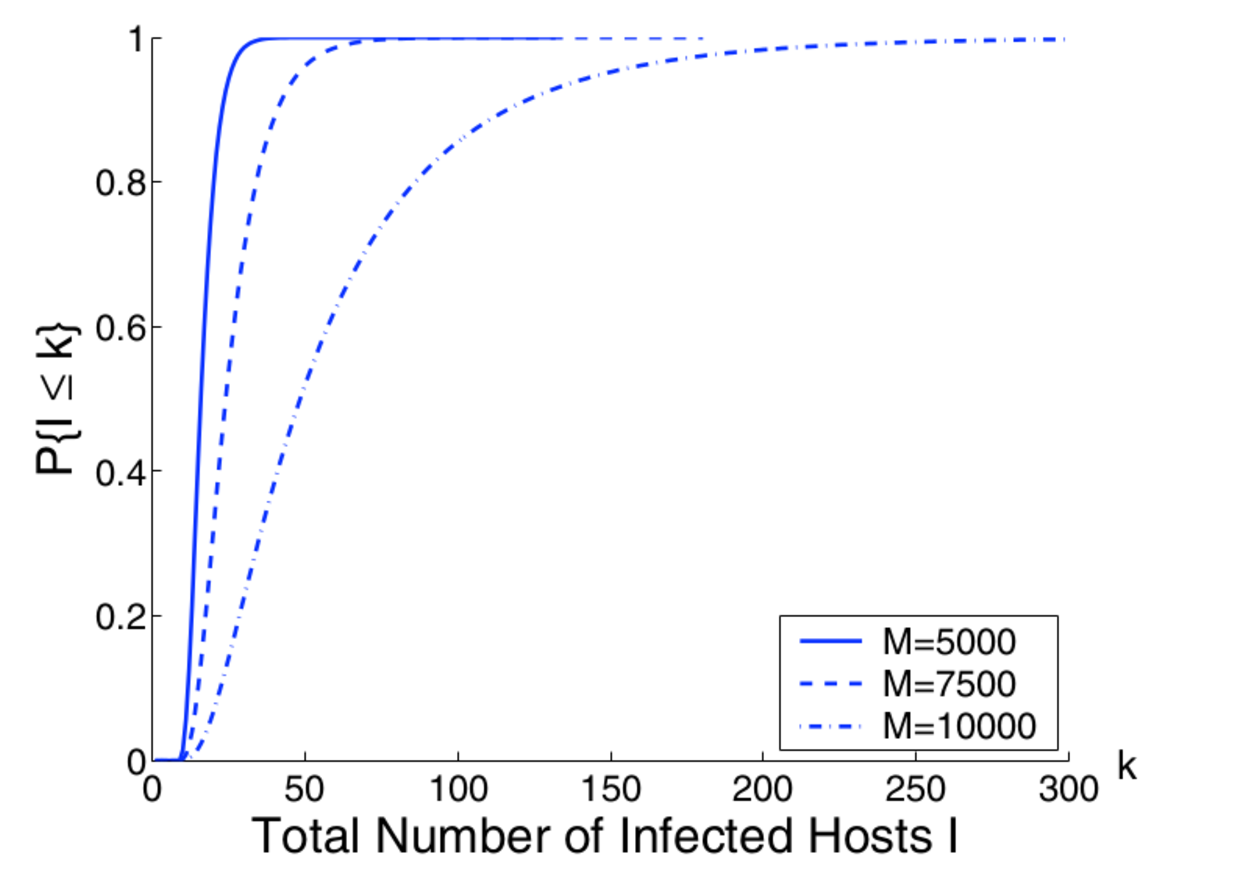
\includegraphics[width=0.6\textwidth]{images/auto.eps}
\caption{distribuzione cumulativa infezioni}
\label{auto}
\end{figure}
In sintesi la strategia si compone dei seguenti passi:
\begin{enumerate}
\item Imporre un limite M al numero di distinti indirizzi IP che un host può contattare in un ciclo di contenimento. All’inizio di ogni ciclo inizializzare il contatore
\item Incrementare il contatore ogni qualvolta viene contattato un nuovo indirizzo IP
\item Se un host raggiunge il valore di soglia prima del termine del ciclo di contenimento viene isolato, analizzato ed eventualmente reso immune prima che venga reintrodotto in rete, dopodiché il contatore viene riazzerato.
\item al termine del ciclo il contatore viene resettato
\end{enumerate}
I vantaggi del contenimento automatizzato sono i seguenti:
\begin{itemize}
\item[-] È una soluzione applicabile a livello di singolo host, quindi semplifica la fase di deploy, inoltre a seconda delle necessità può essere applicata a router di rete impostando un valore di soglia globale per tutti i gli host connessi.
\item[-] Il sistema di contenimento è adatto a worm aventi qualsiasi velocità di scansione, senza conoscerne la signature.
\item[-] Non interferisce con il normale traffico scambiato, poiché dallo studio di Selke et al. emerge che il 97\% degli host contatta meno di 100 indirizzi IP differenti durante un ciclo di contenimento di 30 giorni, soltanto una piccola percentuale raggiunge i 4000 host, pertanto è sufficiente imporre un lower bound al numero di scansioni ponendo M > 5000. Il valore di soglia può comunque essere reso adattivo in base alla normale frequenza di scansionamento dell’host in questione.
\end{itemize}
%%%%%%%%%%%%%%%%%%%%%%%%%%%%%%%%%%%%%%%%%%%%%%%%%%%%%%%%%%%%%%%%%%%%%%%%%%%%%
\subsection{SSL - Security Socket Layer}
L’SSL è un protocollo degli anni ‘90, che ha preceduto il TLS (Transport Layer Security) . Per fornire un meccanismo di autenticazione e cifratura usa una combinazione di cifratura simmetrica e a chiave pubblica. Include i protocolli:
\begin{itemize}
\item[Handshake], in cui viene stabilita una connessione SSL e negoziati algoritmi e sistemi crittografici usati;
\item[Record], in cui si definisce come avviene lo scambio dei dati, quali sono i dati da scambiare e come autenticarli e decifrarli.
\end{itemize}
Siamo interessati al protocollo di Handshake perché implicato direttamente nella fase di diffusione del worm. Secondo tale protocollo:
\begin{itemize}
\item[-] il server presenta il suo certificato digitale al client (certificato X.509);
\item[-] l’autenticazione usa la cifratura a chiave pubblica per validare il certificato digitale;
\item[-] finita l’autenticazione, le parti stabiliscono la cifratura e una chiave di sessione (viene fornita confidenzialità e integrità dei dati).
\end{itemize}
Quindi per abilitare l’SSL, l’admin del web server deve deve ottenere un certificato digitale da una terza parte, cioè un “Autorità di Certificazione”.\\
SSL sarebbe stato la soluzione migliore per evitare la diffusione di Code Red, in quanto questo durante la fase di diffusione andava ad evitare tutti i dispositivi con SSL attivo. L’obiettivo del worm era di raggiungere la più alta diffusione possibile, per poter ottenere un attacco più consistente possibile verso la Casa Bianca.\\
Code Red per infettare nuovi dispositivi agiva nel seguente modo: stabiliva una connessione con un nuovo dispositivo, procedeva con essa e si fermava solo all’inizio di una eventuale fase di handshake, in quanto era sintomo del protocollo SSL attivo, dunque interrompeva la connessione e andava alla ricerca di un nuovo dispositivo da infettare.\\
SSL è un modo semplice per proteggersi da attacchi DDoS, perchè è semplice da implementare e relativamente economico. Richiede solo di possedere un certificato digitale (la cui spesa è di \$349/anno da Verisign Corp.) e una configurazione appropriata.\\
Da un sondaggio del 2001 è emerso purtroppo che meno di 122.000 web server avevano SSL valido, contro i 27 milioni di server attivi (meno della metà dell’1\%). Per questo motivo Code Red non ha trovato freni durante la sua diffusione, e questo è il motivo dell’ingente quantità di macchine che è riuscito ad infettare nel giro di poche ore. Una maggiore attenzione da parte degli amministratori dei server web avrebbe impedito una diffusione cosi estesa, evitando i conseguenti danni registrati.\\
%%%%%%%%%%%%%%%%%%%%%%%%%%%%%%%%%%%%%%%%%%%%%%%%%%%%%%%%%%%%%%%%%%%%%%%%%%%%%
\subsection{ACL - Access Control List}
L’ACL serve per monitorare il traffico, filtrarlo e bloccare un eventuale worm/attacco DDoS. Ne esistono sia per il livello WAN che LAN e sono customizzabili dall’admin. Il loro controllo si basa sull’indirizzo IP del mittente, quindi ogni interfaccia di rete va dotata di un ACL sia per il traffico in ingresso che per quello in uscita.\\
L’ACL rappresenta una misura preventiva per l’attacco e non ha impatto sulle performance del router. L’idea è quella di creare un perimetro entro cui il traffico malevolo non possa entrare, impedendo ai sistemi infetti di attaccare altri sistemi vulnerabili o altre sottoreti. Per tale motivo andrebbero applicate all’interfaccia più vicina alla sorgente di traffico, in modo da avere una maggiore efficienza.\\
Le ACL devono proteggere un server filtrando il traffico, ma devono permette comunque che esso sia accessibile dall’esterno. Quindi le ACL poste al confine delle DMZ devono permettere alle richieste di arrivare ai server, impedendo però che questi siano direttamente accessibili.\\
La strategia per contrastare la diffusione di un worm, o un attacco di tipo DDoS, è quello di isolarlo il prima possibile e procedere alla sua rimozione. Proteggendo la rete con le ACL la minaccia resta confinata in una porzione della rete, e li può essere combattuta ed eliminata con un effort minore rispetto a dopo la sua diffusione.\\
L’impatto di un eventuale attacco DDoS è limitato dal perimetro di rete e gli attaccanti non riescono a raggiungere, ed utilizzare, i dispositivi interni al perimetro a favore dell’attacco. Si evitano sia l’overload dei sistemi che l’interruzione dei servizi basati su tali dispositivi, e di conseguenza che le risorse di rete vengano consumate da traffico non desiderato.\\
Lo svantaggio nell’utilizzo delle ACL è il fatto di doverne usare più di una per aumentare il grado di protezione. Inoltre vanno aggiornate con le vulnerabilità correnti prima dell’eventuale inizio di un attacco, altrimenti non sarebbero in grado di isolarlo tempestivamente.\\
\begin{figure}[!h]
\centering
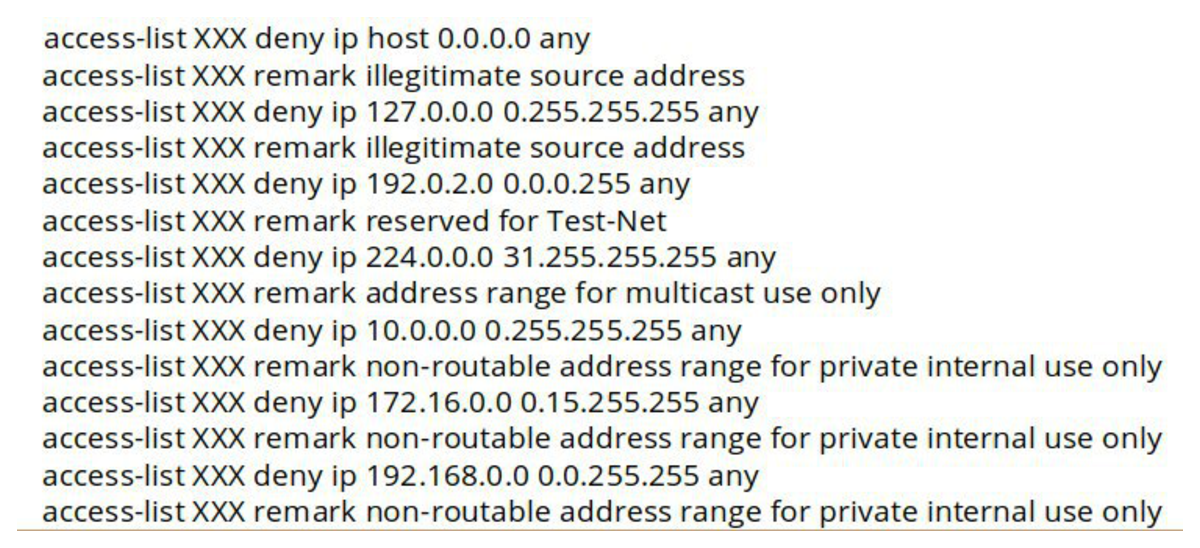
\includegraphics[width=0.6\textwidth]{images/acl.eps}
\caption{esempio di acl}
\label{acl}
\end{figure}
%%%%%%%%%%%%%%%%%%%%%%%%%%%%%%%%%%%%%%%%%%%%%%%%%%%%%%%%%%%%%%%%%%%%%%%%%%%%%
\subsection{Reverse Proxy}
Un server “proxy” è un server che fa da intermediario tra un client ed un altro server, usato per disaccoppiare l’accesso al web da un browser. Le richieste del client non sono gestite direttamente dal server di destinazione ma vengono gestite da un server intermedio.\\
Un server “reverse proxy” viene usato invece come intermediario tra la rete pubblica ed i server ad esso associati. La fase di “three hand handshake” viene eseguita con il reverse proxy ed è lui che inoltrerà la richiesta al web server richiesto.\\
Il reverse proxy è una soluzione adatta per mitigare l’effetto di un attacco DdoS, perchè il traffico malevolo (destinato ad un singolo server) viene distribuito su più reverse proxy.\\
Lo svantaggio nel suo utilizzo è legato al suo costo di mantenimento, nello specifico delle tabelle di configurazione relative ai server web gestiti dal reverse proxy.\\
\begin{figure}[!h]
\centering
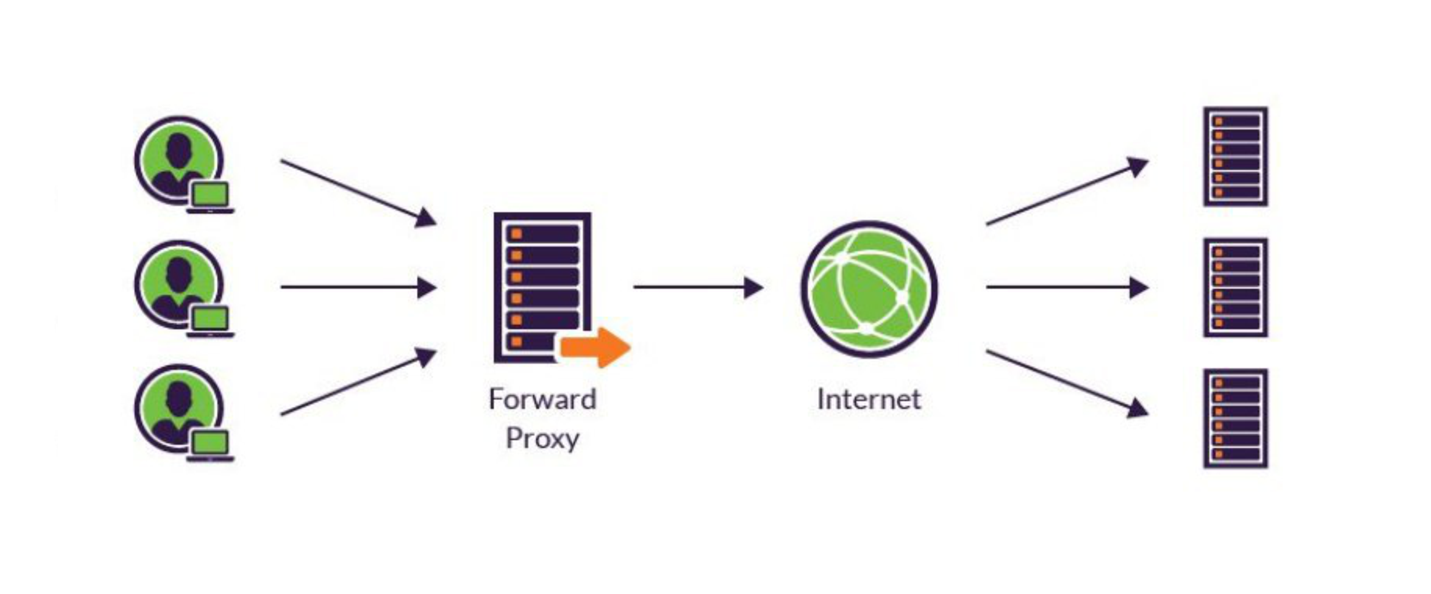
\includegraphics[width=0.6\textwidth]{images/proxy_1.eps}
\caption{esempio forward proxy}
\label{fproxy}
\end{figure}
\begin{figure}[!h]
\centering
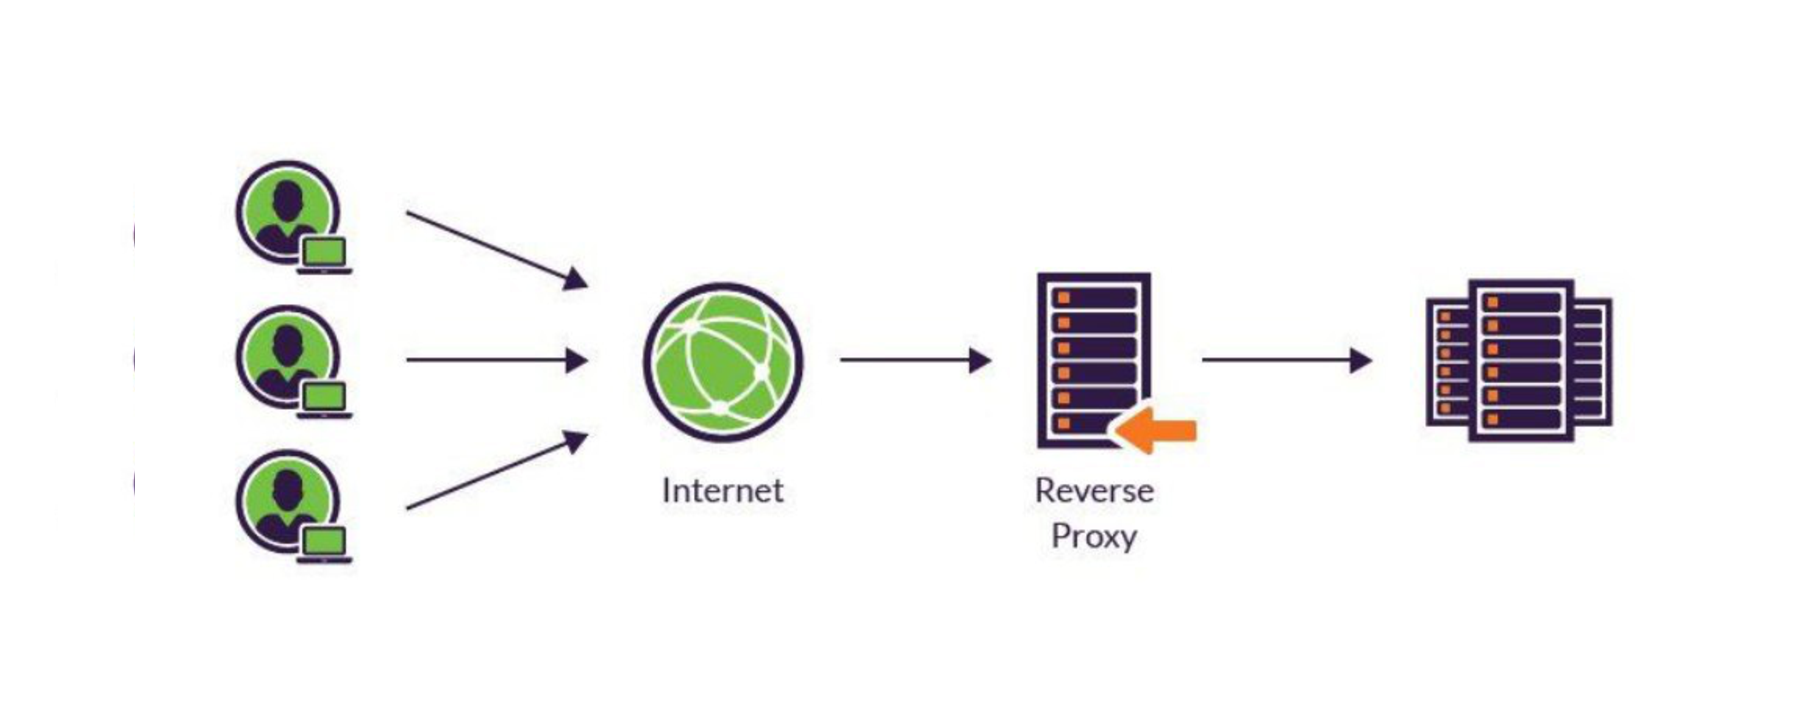
\includegraphics[width=0.6\textwidth]{images/proxy_2.eps}
\caption{esempio reverse proxy}
\label{rproxy}
\end{figure}
%%%%%%%%%%%%%%%%%%%%%%%%%%%%%%%%%%%%%%%%%%%%%%%%%%%%%%%%%%%%%%%%%%%%%%%%%%%%%
\subsection{IDS - Intrusion Detection System}
L’ IDS è un dispositivo hardware o software che colleziona informazioni sul server e/o la rete per analizzarle e determinare la presenza di un attacco o un intrusione.\\
Tale sistema può essere “network-based” se monitora il traffico sul suo segmento di rete, o “host-based” se monitora il software su un server.\\
Può agire a livello di rete, di trasporto o di applicazione ed è in grado di segnalare eventuali anomalie all’admin, o eseguire operazioni in modo autonomo.\\
Per svolgere il suo compito usa come meccanismi:
\begin{itemize}
\item[-]verifica dei log
\item[-]controllo dell’integrità dei file locali
\item[-]monitoring dei pacchetti in arrivo
\end{itemize}
Tale sistema può essere usato in modo molto efficace per contrastare il worm Code Red durante la sua fase di attacco, cioè bloccando l'attacco DdoS sulla porta 80 di un web server. A tal proposito il sistema analizza in real-time le richieste in arrivo al web server, attraverso due tecniche dette “anomaly detection” e “misuse detection”:\\
anomaly detection, confronta le “signature action” con i pattern di intrusione noti che sono contenuti in un database;
misure detection, osserva le operazioni eseguite dal server e costruisce un suo profilo di “utilizzazione normale”, in modo da poter riconoscere operazioni e utilizzi del server diversi da quelli soliti.\\
L’IDS risulta essere molto efficace nel prevenire un attacco, con un elevata affidabilità e ottime performance. Ciò è possibile perché, sfruttando i pattern di attacchi noti, riesce a identificare tempestivamente l’attacco su una macchina, durante le fasi iniziali dell’attacco stesso, riuscendo quindi a impedirne la realizzazione.\\
Lo svantaggio è legato a due fattori principali: il primo è la complessità del sistema stesso, che rende necessaria la presenza di un team di professionisti per configurarlo e utilizzarlo; il secondo è rappresentato dall’utilizzo dei pattern nel database. Infatti quest’ultimo va tenuto sempre aggiornato inserendo manualmente i pattern degli attacchi più recenti, in modo da poterli sfruttare a proprio favore. Inoltre, usando i pattern di attacchi noti, il sistema non è in grado di rilevare un attacco “nuovo” basato su un pattern che non è presente nel database.\\
%%%%%%%%%%%%%%%%%%%%%%%%%%%%%%%%%%%%%%%%%%%%%%%%%%%%%%%%%%%%%%%%%%%%%%%%%%%%%
\subsection{WAF - Web Application Firewall}
Il WAF è un firewall che, a differenza dei firewall di rete, agisce a livello applicativo evitando l’utilizzo delle vulnerabilità di un applicazione. Esso agisce filtrando, monitorando ed eventualmente bloccando il traffico HTTP malevolo.\\
Inoltre ha il vantaggio di essere “customizzabile”, permettendoci di creare un livello di protezione “ad-hoc” per ogni nostra applicazione.\\
Il WAF è una valida alternativa per bloccare/mitigare l’attacco DdoS di Code Red, impedendo che questo possa “bloccare” il target dell’attacco. Infatti degli esperimenti~\cite{sans-acl} del 2004 hanno dimostrato che con soli 500 pacchetti/secondo si poteva bloccare un web server, mentre ne servivano addirittura 14.000 al secondo per riuscire a bloccare un firewall.\\
Utilizzare il WAF ci permette di massimizzare il rilevamento di attacchi noti e non, grazie alla sua analisi dei pacchetti a livello applicativo. Inoltre ha il vantaggio di un impatto minimo sulle performance di rete.\\
Per poter assicurare una maggiore efficacia va usato in combinazione ad un firewall di rete o un IDS. Questo perché il WAF si occupa esclusivamente di una protezione a livello applicativo, lasciando di fatto scoperta una protezione di livello di rete. L’uso di un apposito firewall di rete è una soluzione economica e di facile realizzazione, mentre nel caso ci sia bisogno di una protezione più elevata è utile l’installazione di un più complesso, e costoso, dispositivo IDS.\\
